\chapter{Statistical Physics-Pset1 Solutions}
\begin{abox}
	Practise set-01
\end{abox}
\begin{enumerate}
	\item A particle is confined to the region $x \geq 0$ by a potential which increases linearly as $u(x)=u_{0} x$. The mean position of the particle at temperature $T$ is
	{	\exyear{NET/JRF(JUNE-2011)}}
	\begin{tasks}(2)
		\task[\textbf{a.}] $\frac{k_{B} T}{u_{0}}$
		\task[\textbf{b.}]$\left(k_{B} T\right)^{2} / u_{0}$
		\task[\textbf{c.}]$\sqrt{\frac{k_{B} T}{u_{0}}}$
		\task[\textbf{d.}]  $u_{0} k_{B} T$
	\end{tasks}
	\begin{answer}
		\begin{align*}
		\text{Partition function }Z&=\frac{1}{h} \int e^{-\frac{p^{2}}{2 m k_{B} T}} d p \int e^{-\frac{u_{0} x}{k_{B} T}} d x\text{ and }\langle x\rangle=\int x p(x) d x d p_{x}\\
		\Rightarrow\langle x\rangle&=\frac{\iint x e^{-\frac{p^{2}}{2 m k_{B} T}} d p \cdot e^{\frac{u_{0} x}{k_{B} T}} d x}{\iint e^{\frac{p^{2}}{2 m k_{B} T}} d p \cdot e^{\frac{u_{0} x}{k_{B} T}} d x}=\frac{\int_{0}^{\infty} x e^{\frac{\mu_{0} x}{k_{B} T}} d x}{\int_{0}^{\infty} e^{-\frac{\mu_{0} x}{k_{B} T}} d x}=\frac{\left(\frac{k_{B} T}{u_{0}}\right)^{2}}{\left(\frac{k_{B} T}{u_{0}}\right)} \frac{\int_{0}^{\infty} t e^{-t} d t}{\int_{0}^{\infty} e^{-t} d t}=\frac{k_{B} T}{u_{0}}
		\end{align*}
		So the correct answer is \textbf{Option (a)}
	\end{answer}
	\item 	Consider a system of $N$ non-interacting spins, each of which has classical magnetic moment of magnitude $\mu$. The Hamiltonian of this system in an external magnetic field $\vec{H}$ is $\sum_{i=1}^{N} \vec{\mu}_{i} \cdot \vec{H}$, where $\vec{\mu}_{i}$ is the magnetic moment of the $i^{\text {th }}$ spin. The magnetization per spin at temperature $T$ is
	{	\exyear{NET/JRF(JUNE-2011)}}
	\begin{tasks}(2)
		\task[\textbf{a.}]$\frac{\mu^{2} H}{k_{B} T}$
		\task[\textbf{b.}]$\mu\left[\operatorname{coth}\left(\frac{\mu H}{k_{B} T}\right)-\frac{k_{B} T}{\mu H}\right]$
		\task[\textbf{c.}] $\mu \sinh \left(\frac{\mu H}{k_{B} T}\right)$
		\task[\textbf{d.}] $\mu \tanh \left(\frac{\mu H}{k_{B} T}\right)$
	\end{tasks}
	\begin{answer}
		\begin{align*}
		\text { For classical limit } M&=\frac{\int_{0}^{2 \pi} \int_{0}^{\pi} \mu \cos \theta \exp \frac{\mu H \cos \theta}{k T} \sin \theta d \theta d \phi}{\iint \exp \frac{\mu H \cos \theta}{k_{B} T} \sin \theta d \theta d \phi} \\
		M&=\mu\left[\operatorname{coth}\left(\frac{\mu H}{k_{B} T}\right)-\frac{k_{B} T}{\mu H}\right]
		\end{align*}
		So the correct answer is \textbf{Option (b)}
	\end{answer}
	\item 	The internal energy $E$ of a system is given by $E=\frac{b S^{3}}{V N}$, where $b$ is a constant and other symbols have their usual meaning. The temperature of this system is equal to
	{	\exyear{NET/JRF(DEC-2011)}}
	\begin{tasks}(2)
		\task[\textbf{a.}]$\frac{b S^{2}}{V N}$
		\task[\textbf{b.}]$\frac{3 b S^{2}}{V N}$
		\task[\textbf{c.}]$\frac{b S^{3}}{V^{2} N}$
		\task[\textbf{d.}] $\left(\frac{S}{N}\right)^{2}$
	\end{tasks}
	\begin{answer}
		\begin{align*}
		T d S=d E+P d V \Rightarrow d E=T d S-P d V \Rightarrow\left(\frac{\partial E}{\partial S}\right)_{V}=T \Rightarrow T=\frac{3 b S^{2}}{V N}
		\end{align*}
		So the correct answer is \textbf{Option (b)}
	\end{answer}
	\item A gas of $N$ non-interacting particles is in thermal equilibrium at temperature $T$. Each particle can be in any of the possible non-degenerate states of energy $0,2 \varepsilon$ and $4 \varepsilon$. The average energy per particle of the gas, when $\beta \varepsilon<<1$, is
	{	\exyear{NET/JRF(DEC-2011)}}
	\begin{tasks}(2)
		\task[\textbf{a.}]$2 \varepsilon$
		\task[\textbf{b.}] $3 \varepsilon$
		\task[\textbf{c.}]$2 \varepsilon / 3$
		\task[\textbf{d.}]  $\varepsilon$
	\end{tasks}	
	\begin{answer}
		\begin{align*}
		E_{1}&=0, E_{2}=2 \varepsilon, E_{3}=4 \varepsilon, Z=e^{-0 \beta}+e^{-2 \varepsilon \beta}+e^{-4 \varepsilon \beta} \Rightarrow\langle E\rangle=\frac{0 \cdot e^{-o \beta}+2 \varepsilon e^{-2 \varepsilon \beta}+4 \varepsilon e^{-4 \varepsilon \beta}}{e^{-0 \beta}+e^{-2 \varepsilon \beta}+e^{-4 \varepsilon 1 \beta}} \\
		\Rightarrow\langle E\rangle&=\frac{2 \varepsilon e^{-2 \varepsilon \beta}+4 \varepsilon e^{-4 \varepsilon \beta}}{1+e^{-2 \varepsilon \beta}+e^{-4 \varepsilon \beta}}=\frac{2 \varepsilon(1-2 \varepsilon \beta \ldots .)+4 \varepsilon(1-(4 \varepsilon \beta) \ldots .)}{1+(1-2 \varepsilon \beta \ldots .)+(1-4 \varepsilon \beta \ldots . .)}=\frac{2 \varepsilon+4 \varepsilon}{1+1+1}=\frac{6 \varepsilon}{3}=2 \varepsilon\\
		&\text{	where }\beta \varepsilon<<1.
		\end{align*}
		So the correct answer is \textbf{Option (a)}
	\end{answer}
	\item 	Gas molecules of mass $m$ are confined in a cylinder of radius $R$ and height $L$ (with $R>L$ ) kept vertically in the Earth's gravitational field. The average energy of the gas at low temperatures (such that $m g L \gg k_{B} T$ ) is given by
	{	\exyear{NET/JRF(DEC-2011)}}
	\begin{tasks}(2)
		\task[\textbf{a.}]$N k_{B} T / 2$
		\task[\textbf{b.}]$3 N k_{B} T / 2$
		\task[\textbf{c.}]$2 N k_{B} T$
		\task[\textbf{d.}] $5 N k_{B} T / 2$
	\end{tasks}
	\begin{answer}
		\begin{align*}
		Z&=\frac{1}{h^{3}} \int e^{-\beta H} d p_{x} d p_{y} d p_{z} d x d y d z\\
		Z&=\int_{-\infty}^{\infty} e^{\frac{-p_{x}^{2}}{2 m k_{B} T}} d p_{x} \int_{-\infty}^{\infty} e^{\frac{-p_{y}^{2}}{2 m k_{B} T}} d p_{y} \int_{-\infty}^{\infty} e^{\frac{-p_{z}^{2}}{2 m k_{B} T}} d p_{z} \int d x d y \int_{0}^{L} e^{-\frac{m g z}{k_{B} T}} d z\\
		Z&=\pi R^{2}\left(\frac{m k_{B} T}{2 \pi \hbar^{2}}\right)^{\frac{3}{2}} \int_{0}^{L} e^{-\frac{m g z}{k_{B} T}} d z \Rightarrow Z=\pi R^{2}\left(\frac{m k_{B} T}{2 \pi \hbar^{2}}\right)^{\frac{3}{2}}\left(\frac{1-e^{-\frac{m g L}{k_{B} T}}}{\frac{m g}{k_{B} T}}\right)\\
		Z_{N}&=Z^{N}\\
		\Rightarrow\langle E\rangle&=k_{B} T^{2} \frac{\partial \ln z}{\partial T}=\frac{5 N k_{B} T}{2} \text {, since } m g L>>k_{B} T
		\end{align*}
		So the correct answer is \textbf{Option (d)}
	\end{answer}
	\item 	The free energy of the gas of $N$ particles in a volume $V$ and at a temperature $T$ is $F=N k_{B} T \ln \left[a_{0} V\left(k_{B} T\right)^{5 / 2} / N\right]$, where $a_{0}$ is a constant and $k_{B}$ denotes the Boltzmann constant. The internal energy of the gas is
	{	\exyear{NET/JRF(JUNE-2012)}}
	\begin{tasks}(2)
		\task[\textbf{a.}]$\frac{3}{2} N k_{B} T$
		\task[\textbf{b.}]$\frac{5}{2} N k_{B} T$
		\task[\textbf{c.}]$N k_{B} T \ln \left[a_{0} V\left(k_{B} T\right)^{5 / 2} / N\right]-\frac{3}{2} N k_{B} T$
		\task[\textbf{d.}]  $N k_{B} T \ln \left[a_{0} V /\left(k_{B} T\right)^{5 / 2}\right]$
	\end{tasks}	
	\begin{answer}
		\begin{align*}
		F&=N k_{B} T \ln \left[a_{0} V\left(k_{B} T\right)^{5 / 2} / N\right], F=U-T S, U=F+T S\\
		d F&=-S d T-P d V \Rightarrow\left(\frac{\partial F}{\partial T}\right)_{V}=-S \text { or } S=-\left(\frac{\partial F}{\partial T}\right)_{V} \Rightarrow U=F-T\left(\frac{\partial F}{\partial T}\right)_{V} \\
		F&=N k_{B} T \ln \left(C T^{5 / 2}\right) \text { where } C=\frac{a_{0} V k_{B}^{5 / 2}}{N} \\
		\left(\frac{\partial F}{\partial T}\right)_{V}&=N k_{B} \ln \left(C T^{5 / 2}\right)+N k_{B} T \frac{C}{C T^{5 / 2}} \frac{5}{2} T^{3 / 2} \Rightarrow T\left(\frac{\partial F}{\partial T}\right)_{V}=N k_{B} T \ln \left(C T^{5 / 2}\right)+\frac{5}{2} N k_{B} T \\
		T\left(\frac{\partial F}{\partial T}\right)_{V}&=F+\frac{5}{2} N k_{B} T \Rightarrow U=F-T\left(\frac{\partial F}{\partial T}\right)_{V}=-\frac{5}{2} N k_{B} T .\\
		T\left(\frac{\partial F}{\partial T}\right)_{V}&=F+\frac{5}{2} N k_{B} T \Rightarrow U=F-T\left(\frac{\partial F}{\partial T}\right)_{V}=-\frac{5}{2} N k_{B} T .
		\end{align*}
		So the correct answer is \textbf{Option (b)}
	\end{answer}
	\item A system has two normal modes of vibration, with frequencies $\omega_{1}$ and $\omega_{2}=2 \omega_{1}$. What is the probability that at temperature $T$, the system has an energy less than $4 \hbar \omega_{1}$ ?
	[In the following $x=e^{-\beta \hbar \omega_{1}}$ and $Z$ is the partition function of the system.]
	{	\exyear{NET/JRF(JUNE-2012)}}
	\begin{tasks}(2)
		\task[\textbf{a.}]$x^{3 / 2}\left(x+2 x^{2}\right) / Z$
		\task[\textbf{b.}]$x^{3 / 2}\left(1+x+x^{2}\right) / Z$
		\task[\textbf{c.}]$x^{3 / 2}\left(1+2 x^{2}\right) / Z$
		\task[\textbf{d.}] $x^{3 / 2}\left(1+x+2 x^{2}\right) / Z$
	\end{tasks}
	\begin{answer}
		\begin{align*}
		\intertext{There is two normal mode so there is two degree of freedom.}
		\intertext{	Energy of harmonic oscillator is $E=\left(n_{1}+\frac{1}{2}\right) \hbar \omega_{1}+\left(n_{2}+\frac{1}{2}\right) \hbar \omega_{2}$.} E&=\left(n_{1}+\frac{1}{2}\right) \hbar \omega_{1}+\left(n_{2}+\frac{1}{2}\right) \hbar 2 \omega_{1}\text{ where } n_{1}=0,1,2,3 \ldots .
		\text{ and }n_{2}=0,1,2,3 \ldots .\\
		\intertext{	Ground state energy $E=\frac{3 \hbar \omega_{1}}{2}$, first excited state energy $E=\frac{5 \hbar \omega_{1}}{2}$. Second excited state energy $E=\frac{7 \hbar \omega_{1}}{2}$ which is doubly degenerate state so $g=2$, other state have more energy than $4 \hbar \omega_{1}$.}
		P\left(E<4 \hbar \omega_{1}\right)&=\frac{e^{-\frac{3 \beta \hbar \omega_{1}}{2}}+e^{-\frac{5 \beta \hbar \omega_{1}}{2}}+2 e^{-\frac{7 \beta \hbar \omega_{1}}{2}}}{Z}=\frac{x^{3 / 2}\left(1+x+2 x^{2}\right)}{Z}\text{ where }x=e^{-\beta \hbar \omega_{1}} .
		\end{align*}
		So the correct answer is \textbf{Option (d)}
	\end{answer}
	\item 	The entropy of a system, $(S)$, is related to the accessible phase space volume $\Gamma$ by $S=k_{B} \ln \Gamma(E, N, V)$ where $E, N$ and $V$ are the energy, number of particles and volume respectively. From this one can conclude that $\Gamma$
	{	\exyear{NET/JRF(DEC-2012)}}
	\begin{tasks}(2)
		\task[\textbf{a.}]does not change during evolution to equilibrium
		\task[\textbf{b.}]oscillates during evolution to equilibrium
		\task[\textbf{c.}]is a maximum at equilibrium
		\task[\textbf{d.}]is a minimum at equilibrium 
	\end{tasks}
	\begin{answer}
		Entropy is maximum at equilibrium.\\
		So the correct answer is \textbf{Option (c)}
	\end{answer}
	\item 	Consider a one-dimensional Ising model with $N$ spins, at very low temperatures when almost all spins are aligned parallel to each other. There will be a few spin flips with each flip costing an energy $2 J$. In a configuration with $r$ spin flips, the energy of the system is $E=-N J+2 r J$ and the number of configuration is ${ }^{N} C_{r} ; r$ varies from 0 to $N$. The partition function is
	{	\exyear{NET/JRF(DEC-2012)}}
	\begin{tasks}(2)
		\task[\textbf{a.}] $\left(\frac{J}{k_{B} T}\right)^{N}$
		\task[\textbf{b.}]$e^{-N J / k_{B} T}$
		\task[\textbf{c.}] $\left(\sinh \frac{J}{k_{B} T}\right)^{N}$
		\task[\textbf{d.}] $\left(\cosh \frac{J}{k_{B} T}\right)^{N}$
	\end{tasks}
	\begin{answer}
		\begin{align*}
		\text { Let us}&\text{ consider only three energy levels, } E_{r}=-2 J+2 r J \text { i.e. } E_{0}=-2 J, E_{1}=0 \text { and }\\
		E_{2}&=2 J.\\
		Q_{2}&=\frac{\left({ }^{2} C_{0} e^{-\beta E_{0}}+{ }^{2} C_{1} e^{-\beta E_{1}}+{ }^{2} C_{2} e^{-\beta E_{2}}\right)}{\sum_{r=0}^{2}{ }^{2} C_{r}}=\frac{\left(e^{\beta 2 J}+2 e^{0}+e^{\beta 2 J}\right)}{4}=\frac{\left(e^{\beta J}+e^{\beta J}\right)^{2}}{4} \\
		Q_{2}&=\left(\frac{e^{\beta J}+e^{\beta J}}{2}\right)^{2}=(\cosh \beta J)^{2} \Rightarrow(\cosh \beta J)^{2} \Rightarrow Q_{N}=(\cosh \beta J)^{N}
		\end{align*}
		So the correct answer is \textbf{Option (d)}
	\end{answer}
	\item Consider a system of three spins $S_{1}, S_{2}$ and $S_{3}$ each of which can take values $+1$ and $-1$. The energy of the system is given by $E=-J\left[S_{1} S_{2}+S_{2} S_{3}+S_{3} S_{1}\right]$ where $J$ is a positive constant. The minimum energy and the corresponding number of spin configuration are, respectively,
	{	\exyear{NET/JRF(DEC-2012)}}
	\begin{tasks}(2)
		\task[\textbf{a.}]$J$ and 1
		\task[\textbf{b.}]$-3 J$ and 1
		\task[\textbf{c.}]$-3 J$ and 2
		\task[\textbf{d.}]  $-6 J$ and 2
	\end{tasks}
	\begin{answer}
		\begin{align*}
		\text{If we take }S_{1}&=S_{2}=S_{3}=+1\text{ i.e. }\hspace{3cm}\stackrel{\uparrow}{s_1}\qquad \stackrel{\uparrow}{s_2}\qquad\stackrel{\uparrow}{s_3}\\
		\text { Then energy, } E&=-J[1 \times 1+1 \times 1+1 \times 1]=-3 J\\
		\text { Again } S_{1}&=S_{2}=S_{3}=-1 \text {, then }\hspace{2.8cm}\downarrow\qquad \ \downarrow\qquad \ \downarrow\\
		\text{Energy }(E)&=-3 J
		\intertext{So, minimum energy is $(-3 J)$ and there are two spin configuration.}\\
		\text { If we take }&\stackrel{\uparrow}{s_1}\qquad \stackrel{\downarrow}{s_2}\qquad\stackrel{\uparrow}{s_3}\\
		\text { Then we get Maximum energy } E&=J \text {. }
		\end{align*}
		So the correct answer is \textbf{Option (c)}
	\end{answer}
	\item 	Consider a system of two Ising spins $S_{1}$ and $S_{2}$ taking values $\pm 1$ with interaction energy given by $\varepsilon=-J S_{1} S_{2}$, when it is in thermal equilibrium at temperature $T$. For large $T$, the average energy of the system varies as $C / k_{B} T$, with $C$ given by
	{	\exyear{NET/JRF(JUNE-2013)}}
	\begin{tasks}(2)
		\task[\textbf{a.}]$-2 J^{2}$
		\task[\textbf{b.}] $-J^{2}$
		\task[\textbf{c.}]$J^{2}$
		\task[\textbf{d.}] $4 J$ 
	\end{tasks}
	\begin{answer}
		\begin{align*}
		\intertext{The interaction energy is given by $E=-J S_{1} S_{2}$ where $S_{1}$ and $S_{2}$ taking values $\pm 1$.}
		\text { Possible }&\text{values of the Energy of the system are }\\
		E_{1}&=-J 1 \cdot 1=-J, \quad E_{2}=-J(-1) \cdot(1)=+J\\
		E_{3}&=-J(1) \cdot(-1)=+J, \quad E_{4}=-J(-1) \cdot(-1)=-J\\
		\langle U\rangle&=\frac{\sum_{r} E_{r} g_{r} e^{-\frac{E_{r}}{k T}}}{\sum_{r} g_{r} e^{\frac{E_{r}}{k T}}}=\frac{-2 J e^{\frac{J}{k T}}+2 J e^{\frac{J}{k T}}}{2 e^{\frac{J}{k T}}+2 e^{-\frac{J}{k T}}}=-J\left(\frac{e^{\frac{J}{k T}}-e^{-\frac{J}{k T}}}{e^{\frac{J}{k T}}+e^{\frac{J}{k T}}}\right)=-J \frac{\left(1+\frac{J}{k T}-\left(1-\frac{J}{k T}\right)\right)}{1+\left(\frac{J}{k T}\right)+1-\left(\frac{J}{k T}\right)}\\
		\Rightarrow\langle U\rangle&=-\frac{J^{2}}{k T} \Rightarrow C=-J^{2} \quad \text { (For large } T, \frac{J}{k T}<<1 \text { ) }
		\end{align*}
		So the correct answer is \textbf{Option (b)}
	\end{answer}
	\item A collection $N$ of non-interacting spins $S_{i}, i=1,2, \ldots \ldots, N,\left(S_{i}=\pm 1\right)$ is kept in an external magnetic field $B$ at a temperature $T$. The Hamiltonian of the system is $H=-\mu B \Sigma_{i} S_{i}$. What should be the minimum value of $\frac{\mu B}{k_{B} T}$ for which the mean value $\left\langle S_{i}\right\rangle \geq \frac{1}{3}$ ?
	{	\exyear{NET/JRF(DEC-2014)}}
	\begin{tasks}(2)
		\task[\textbf{a.}]$\frac{1}{2} N \ln 2$
		\task[\textbf{b.}] $2 \ln 2$
		\task[\textbf{c.}]$\frac{1}{2} \ln 2$
		\task[\textbf{d.}] $N \ln 2$	
	\end{tasks}	
	\begin{answer}
		\begin{align*}
		P\left(S_{i}=+1\right)&=\frac{e^{-\frac{\mu B}{k T}}}{e^{-\frac{\mu B}{k T}}+e^{\frac{\mu B}{k T}}}, P\left(S_{i}=-1\right)=\frac{e^{\frac{\mu B}{k T}}}{e^{-\frac{\mu B}{k T}}+e^{\frac{\mu B}{k T}}}\\
		\left\langle S_{i}\right\rangle&=\frac{+1 e^{-\frac{\mu B}{k T}}-e^{+\frac{\mu B}{k T}}}{e^{-\frac{\mu B}{k T}}+e^{\frac{\mu B}{k T}}} \Rightarrow\left\langle S_{i}\right\rangle=-\left(\tanh \frac{\mu B}{k T}\right)\\
		\text{For $N$ particle }&\left\langle S_{i}\right\rangle=-N \tanh \frac{\mu B}{k T}\\
		\text{	According to question, }&\frac{\left\langle S_{i}\right\rangle}{N} \geq \frac{1}{3} \Rightarrow-\tanh \left(\frac{\mu B}{k T}\right)=\frac{1}{3} \Rightarrow \frac{\mu B}{k T}=\frac{1}{2} \ln 2
		\end{align*}
		So the correct answer is \textbf{Option (c)}
	\end{answer}
	\item A system of $N$ distinguishable particles, each of which can be in one of the two energy levels 0 and $\in$, has a total energy $n \in$, where $n$ is an integer. The entropy of the system is proportional to
	{	\exyear{NET/JRF(JUNE-2015)}}
	\begin{tasks}(2)
		\task[\textbf{a.}]$N \ln n$
		\task[\textbf{b.}]$n \ln N$
		\task[\textbf{c.}] $\ln \left(\frac{N !}{n !}\right)$
		\task[\textbf{d.}] $\ln \left(\frac{N !}{n !(N-n) !}\right)$
	\end{tasks}
	\begin{answer}
		\begin{align*}
		??
		\end{align*}
		So the correct answer is \textbf{Option (d)}
	\end{answer}
	\item Consider three Ising spins at the vertices of a triangle which interact with each other with a ferromagnetic Ising interaction of strength $J$. The partition function of the system at temperature $T$ is given by $\left(\beta=\frac{1}{k_{B} T}\right)$ :
	{	\exyear{NET/JRF(JUNE-2015)}}
	\begin{tasks}(2)
		\task[\textbf{a.}] $2 e^{3 \beta J}+6 e^{-\beta J}$
		\task[\textbf{b.}] $2 e^{-3 \beta J}+6 e^{\beta J}$
		\task[\textbf{c.}]$2 e^{3 \beta J}+6 e^{-3 \beta J}+3 e^{\beta J}+3 e^{-\beta J}$
		\task[\textbf{d.}] $(2 \cosh \beta J)^{3}$
	\end{tasks}
	\begin{answer}
		\begin{align*}
		&H=J\left(S_{1} S_{2}+S_{1} S_{3}+S_{2} S_{3}\right)\\
		&\begin{array}{llll}
		S_{1} & S_{2} & S_{3} & E
		\end{array}\\
		&\begin{array}{llll}
		1 & 1 & 1 & 3 J
		\end{array}\\
		&\left.\begin{array}{ccc}
		1 & 1 & -1 \\
		1 & -1 & 1 \\
		-1 & 1 & 1
		\end{array}\right\}-J\\
		&\begin{array}{lll}
		-1 & -1 & 1
		\end{array}\\
		&\left.\begin{array}{ccc}
		-1 & 1 & -1 \\
		1 & -1 & -1
		\end{array}\right\}-J\\
		&\left.\begin{array}{lll}
		-1 & -1 & -1
		\end{array}\right\} 3 J\\
		\Rightarrow&z=2 e^{-3 \beta J}+6 e^{\beta J}
		\end{align*}
		So the correct answer is \textbf{Option (b)}
	\end{answer}
	\item The partition function of a system of $N$ Ising spins is $Z=\lambda_{1}^{N}+\lambda_{2}^{N}$ where $\lambda_{1}$ and $\lambda_{2}$ are functions of temperature, but are independent of $N$. If $\lambda_{1}>\lambda_{2}$, the free energy per spin in the limit $N \rightarrow \infty$ is
	{	\exyear{NET/JRF(DEC-2015)}}
	\begin{tasks}(2)
		\task[\textbf{a.}]$-k_{B} T \ln \left(\frac{\lambda_{1}}{\lambda_{2}}\right)$
		\task[\textbf{b.}] $-k_{B} T \ln \lambda_{2}$
		\task[\textbf{c.}]$-k_{B} T \ln \left(\lambda_{1} \lambda_{2}\right)$
		\task[\textbf{d.}] $-k_{B} T \ln \lambda_{1}$
	\end{tasks}
	\begin{answer}
		\begin{align*}
		Z&=\lambda_{1}^{N}+\lambda_{2}^{N}, F=-k T \ln \left(\lambda_{1}^{N}+\lambda_{2}^{N}\right)\text{, it is given } \lambda_{1}>>\lambda_{2}\\
		\Rightarrow F&=-k T \ln \left[\lambda_{1}^{N}\left(1+\left(\frac{\lambda_{2}}{\lambda_{1}}\right)^{N}\right], \quad \frac{\lambda_{2}}{\lambda_{1}} \approx 0\right. \\
		F&=-k T \ln \lambda_{1}^{N}=-N k T \ln \lambda_{1} \Rightarrow \frac{F}{N}=-k T \ln \lambda_{1}
		\end{align*}
		So the correct answer is \textbf{Option (d)}
	\end{answer}
	\item The Hamiltonian of a system of $N$ non interacting spin $\frac{1}{2}$ particles is $H=-\mu_{0} B \sum_{i} S_{i}^{z}$, where $S_{i}^{z}=\pm 1$ are components of $i^{\text {th }}$ spin along an external magnetic field $B$. At a temperature $T$ such that $e^{\frac{\mu_{0} B}{k_{B} T}}=2$. the specific heat per particle is
	{	\exyear{NET/JRF(DEC-2015)}}
	\begin{tasks}(2)
		\task[\textbf{a.}]$\frac{16}{25} k_{B}$
		\task[\textbf{b.}] $\frac{8}{25} k_{B} \ln 2$
		\task[\textbf{c.}]$k_{B}(\ln 2)^{2}$
		\task[\textbf{d.}]  $\frac{16}{25} k_{B}(\ln 2)^{2}$
	\end{tasks}
	\begin{answer}
		\begin{align*}
		\text {  For the given system } E&=-\mu_{0} B \tanh \frac{\mu_{0} B}{k T}\\
		C_{V}&=\left(\frac{\mu_{0} B}{k T}\right)^{2} N k \sec ^{2} h \frac{\mu_{0} B}{k T}\\
		\frac{C_{V}}{N}&=\left(\frac{\mu_{0} B}{k T}\right)^{2} k \frac{4}{\left(e^{\frac{\mu_{0} B}{k T}}+e^{-\frac{\mu_{0} B}{k T}}\right)^{2}} \quad \because e^{\frac{\mu_{0} B}{k T}}=2 \Rightarrow \frac{\mu_{0} B}{k T}=\ln 2\\
		\frac{C_{V}}{N}&=\left(\frac{\mu_{0} B}{k T}\right)^{2} k \frac{4}{\left(2+\frac{1}{2}\right)^{2}}=\left(\frac{\mu_{0} B}{k T}\right)^{2} k \frac{16}{25}=(\ln 2)^{2} \frac{16 k}{25}=\frac{16}{25} k(\ln 2)^{2}
		\end{align*}
		So the correct answer is \textbf{Option (d)}
	\end{answer}
	\item A gas of non-relativistic classical particles in one dimension is subjected to a potential $V(x)=\alpha|x|$ (where $\alpha$ is a constant). The partition function is $\left(\beta=\frac{1}{k_{B} T}\right)$
	{	\exyear{NET/JRF(JUNE-2016)}}
	\begin{tasks}(2)
		\task[\textbf{a.}] $\sqrt{\frac{4 m \pi}{\beta^{3} \alpha^{2} h^{2}}}$
		\task[\textbf{b.}] $\sqrt{\frac{2 m \pi}{\beta^{3} \alpha^{2} h^{2}}}$
		\task[\textbf{c.}]$\sqrt{\frac{8 m \pi}{\beta^{3} \alpha^{2} h^{2}}}$
		\task[\textbf{d.}] $\sqrt{\frac{3 m \pi}{\beta^{3} \alpha^{2} h^{2}}}$
	\end{tasks}
	\begin{answer}
		\begin{align*}
		z&=\frac{1}{h} \int_{-\infty}^{\infty} e^{-\frac{p_{x}^{2}}{2 m k T}} d p_{x} \int_{-\infty}^{\infty} e^{-\frac{\alpha|x|}{k T}} d x=\frac{1}{h}(2 \pi m k T)^{1 / 2} \int_{-\infty}^{\infty} e^{\frac{\alpha|x|}{k T}} d x\\
		\Rightarrow z&=\left(\frac{2 \pi m k T}{h^{2}}\right)^{1 / 2} \int_{-\infty}^{\infty} e^{-\frac{\alpha|x|}{k T}} d x\\
		\because \int_{-\infty}^{\infty} e^{-\frac{\alpha|x|}{k T}} d x&=\int_{-\infty}^{0} e^{+\frac{\alpha x}{k T}} d x+\int_{0}^{\infty} e^{-\frac{\alpha x}{k T}} d x=\frac{k T}{\alpha}+\frac{k T}{\alpha}=\frac{2 k T}{\alpha}\\
		z&=\left(\frac{2 \pi m k T}{h^{2}}\right)^{1 / 2}\left(\frac{2 k T}{\alpha}\right)=\left(\frac{8 \pi m}{h^{2} \beta^{3} \alpha^{2}}\right)^{\frac{1}{2}}\qquad
		\text{	put }\beta=\frac{1}{k T}
		\end{align*}
		So the correct answer is \textbf{Option (c)}
	\end{answer}
	\item Consider a random walk on an infinite two-dimensional triangular lattice, a part of which is shown in the figure below.
	\begin{figure}[H]
		\centering
		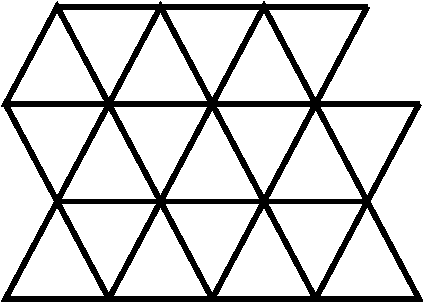
\includegraphics[height=3cm,width=4cm]{SP-11}
	\end{figure}
	If the probabilities of moving to any of the nearest neighbour sites are equal, what is the probability that the walker returns to the starting position at the end of exactly three steps?
	{	\exyear{NET/JRF(DEC-2016)}}
	\begin{tasks}(2)
		\task[\textbf{a.}]$\frac{1}{36}$
		\task[\textbf{b.}]$\frac{1}{216}$
		\task[\textbf{c.}] $\frac{1}{18}$
		\task[\textbf{d.}] $\frac{1}{12}$
	\end{tasks}
	\begin{answer}
		Solution: For walker to return to starting position it must move along an equivalent triangle in three steps.\\
		For steps one any movement can result in equilateral triangle.\\
		For step two, two out of six options will form equilateral triangle.\\
		For step three, only one out of six options will form equilateral\\ triangle Total probability $=\frac{6}{6} \times \frac{2}{6} \times \frac{1}{6}=\frac{1}{18}$\\
		So the correct answer is \textbf{Option (c)}
	\end{answer}
	\item 	An atom has a non-degenerate ground-state and a doubly-degenerate excited state. The energy difference between the two states is $\varepsilon$. The specific heat at very low temperatures $(\beta \varepsilon \gg 1)$ is given by
	{	\exyear{NET/JRF(DEC-2016)}}
	\begin{tasks}(2)
		\task[\textbf{a.}]$k_{B}(\beta \varepsilon)$
		\task[\textbf{b.}]$k_{B} e^{-\beta \varepsilon}$
		\task[\textbf{c.}] $2 k_{B}(\beta \varepsilon)^{2} e^{-\beta \varepsilon}$
		\task[\textbf{d.}]  $k_{B}$
	\end{tasks}
	\begin{answer}
		\begin{align*}
		\intertext{Assume energy at ground state is 0 and energy at first excited state is $\in$. The partition function is $Z=1+2 e^{-\beta \epsilon}$}
		\text{	Energy }&=\frac{2 \in e^{-\beta \epsilon}}{\left(1+2 e^{-\beta \epsilon}\right)}\\
		\text{Specific heat, }C_{V}&=\left(\frac{\partial U}{\partial T}\right)_{V}=\frac{2 \in e^{-\frac{\epsilon}{k T}}(-\in) \frac{-1}{k T^{2}}}{\left(1+2 e^{\frac{-\epsilon}{k T}}\right)}+\frac{2 \in e^{\frac{-\epsilon}{k T}} \in \in \frac{2}{k T^{2}}}{\left(1+2 e^{\frac{-\epsilon}{k T}}\right)^{2}}\\
		&=2 k\left(\frac{\epsilon}{k T}\right)^{2} e^{\frac{-\epsilon}{k T}} \frac{\left(1+2 e^{\frac{-\epsilon}{k T}}\right)}{\left(1+2 e^{\frac{-\epsilon}{k T}}\right)^{2}}=2 k(\beta \in)^{2} e^{-\beta \in} \frac{\left(1+2 e^{-\beta \epsilon}\right)}{\left(1+2 e^{-\beta \epsilon}\right)^{2}}\\
		C_{V} &\simeq 2 k(\beta \in)^{2} e^{-\beta \epsilon}, \quad \beta \in \rightarrow \infty
		\end{align*}
		So the correct answer is \textbf{Option (c)}
	\end{answer}
	\item In a thermodynamic system in equilibrium, each molecule can exist in three possible states with probabilities $1 / 2,1 / 3$ and $1 / 6$ respectively. The entropy per molecule is
	{	\exyear{NET/JRF(JUNE-2017)}}
	\begin{tasks}(2)
		\task[\textbf{a.}] $k_{B} \ln 3$
		\task[\textbf{b.}]$\frac{1}{2} k_{B} \ln 2+\frac{2}{3} k_{B} \ln 3$
		\task[\textbf{c.}]$\frac{2}{3} k_{B} \ln 2+\frac{1}{2} k_{B} \ln 3$
		\task[\textbf{d.}] $\frac{1}{2} k_{B} \ln 2+\frac{1}{6} k_{B} \ln 3$
	\end{tasks}
	\begin{answer}
		\begin{align*}
		S&=-k_{B} \sum_{i} P i \ln P i\\
		P_{1}&=\frac{1}{2}, P_{2}=1 / 3 \text { and } P_{3}=1 / 6 \\
		S&=-k_{B}\left(\frac{1}{2} \ln 1 / 2+1 / 3 \ln 1 / 3+1 / 6 \ln 1 / 6\right) . \\
		&=-k_{b}\left(\frac{1}{2}(\ln 1-\ln 2)+\frac{1}{3}(\ln 1-\ln 3)+\frac{1}{6}(\ln 1-\ln 6)\right. \\
		&=k_{B}\left[\frac{1}{2} \ln 2+\frac{1}{3} \ln 3+\frac{1}{6} \ln 2+\frac{1}{6} \ln 3\right]=k_{B}\left[\frac{1}{2} \ln 2+\frac{1}{6} \ln 2+\frac{1}{3} \ln 3+\frac{1}{6} \ln 3\right] \\
		S&=k_{B}\left[\frac{3 \ln 2+\ln 2}{6}+\frac{2 \ln 3+\ln 3}{6}\right]=k_{B}\left(\frac{4 \ln 2}{6}+\frac{3 \ln 3}{6}\right)=k_{B}\left[\frac{2}{3} \ln 2+\frac{1}{2} \ln 3\right]
		\end{align*}
		So the correct answer is \textbf{Option (c)}
	\end{answer}
\end{enumerate}
\newpage
\begin{abox}
	Practise set-2
\end{abox}
\begin{enumerate}
	\item A system of $\mathrm{N}$ non-interacting classical point particles is constrained to move on the twodimensional surface of a sphere. The internal energy of the system is
	{\exyear{GATE 2010}}
	\begin{tasks}(4)
		\task[\textbf{A.}] $\frac{3}{2} N k_{B} T$
		\task[\textbf{B.}] $\frac{1}{2} N k_{B} T$
		\task[\textbf{C.}] $N k_{B} T$
		\task[\textbf{D.}] $\frac{5}{2} N k_{B} T$
	\end{tasks}
	\begin{answer}
		\begin{align*}
		\text{There are $2 \mathrm{~N}$ degree of freedom.}\\
		\text{The internal energy of the system is}\frac{N k_{B} T}{2}+\frac{N k_{B} T}{2}&=N k_{B} T
		\end{align*}
		So the correct answer is \textbf{Option (C)}
	\end{answer}
	\item Partition function for a gas of photons is given as, $\ln Z=\frac{\pi^{2} V\left(k_{B} T\right)^{3}}{45 \hbar^{3} C^{3}}$. The specific heat of the photon gas varies with temperature as
	{\exyear{GATE 2010}}
	\begin{tasks}(2)
		\task[\textbf{A.}] \begin{figure}[H]
			\centering
			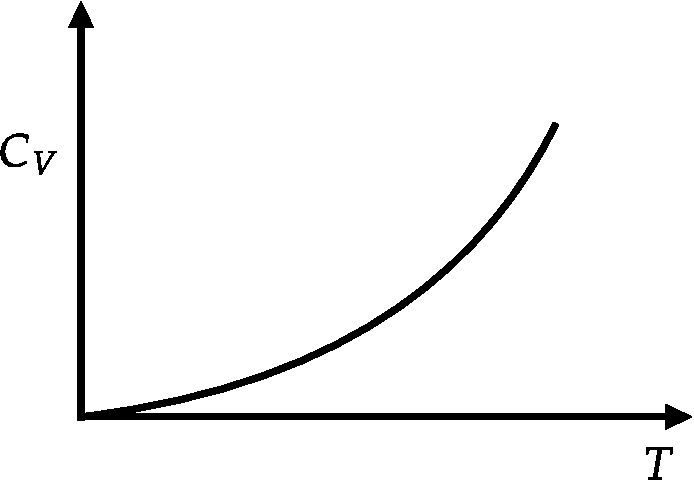
\includegraphics[height=3cm,width=4.5cm]{diagram-20210910(14)-crop}
		\end{figure}
		\task[\textbf{B.}] \begin{figure}[H]
			\centering
			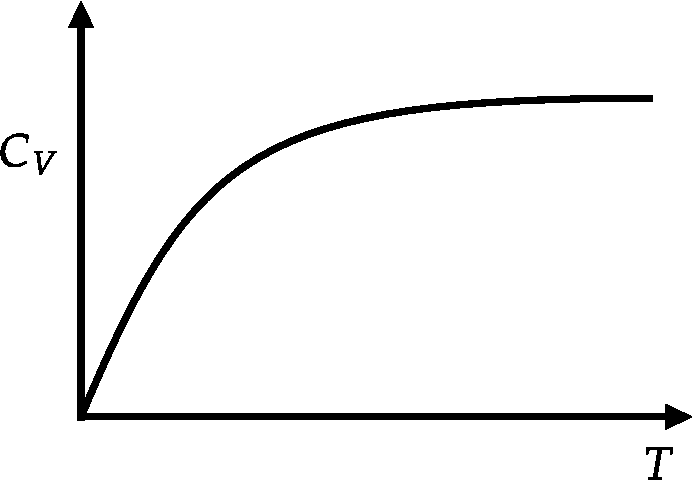
\includegraphics[height=3cm,width=4.5cm]{diagram-20210910(15)-crop}
		\end{figure}
		\task[\textbf{C.}] \begin{figure}[H]
			\centering
			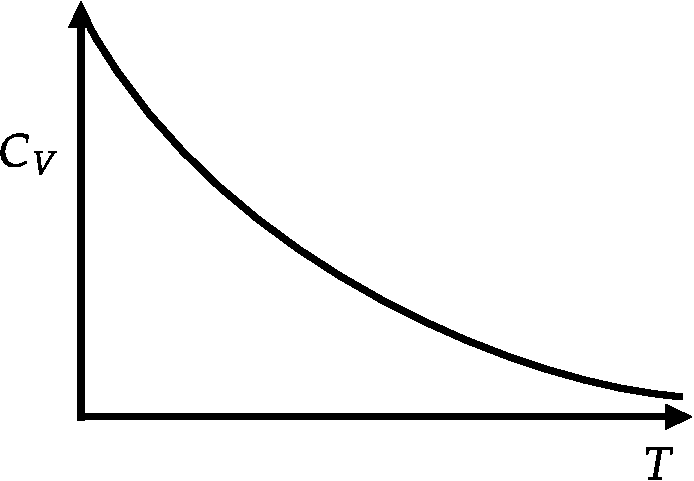
\includegraphics[height=3cm,width=4.5cm]{diagram-20210910(16)-crop}
		\end{figure}
		\task[\textbf{D.}] \begin{figure}[H]
			\centering
			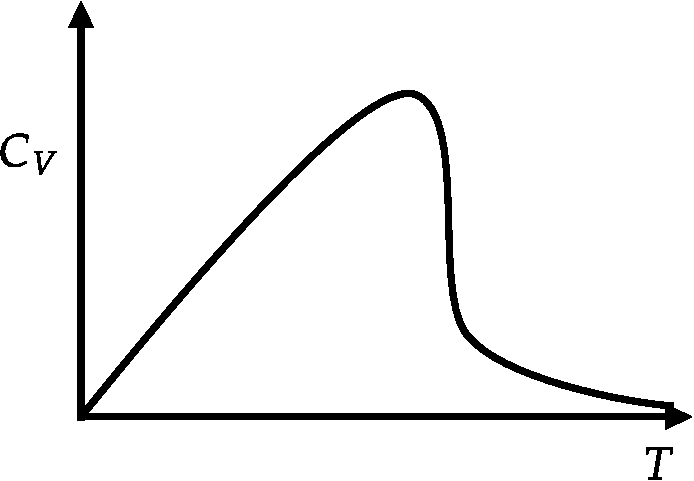
\includegraphics[height=3cm,width=4.5cm]{diagram-20210910(17)-crop}
		\end{figure}
	\end{tasks}
	\begin{answer}
		\begin{align*}
		\mathrm{U}=\mathrm{K}_{\mathrm{B}} \mathrm{T}^{2} \frac{\partial \ln \mathrm{z}}{\partial \mathrm{T}}, \quad \mathrm{C}_{\mathrm{v}}=\left(\frac{\partial \mathrm{U}}{\partial \mathrm{T}}\right)_{\mathrm{v}} \Rightarrow \mathrm{C}_{\mathrm{v}} \propto \mathrm{T}^{3}
		\end{align*}
		So the correct answer is \textbf{Option (A)}
	\end{answer}
	\item From Q. no. 2, the pressure of the photon gas is
	{\exyear{GATE 2010}}
	\begin{tasks}(4)
		\task[\textbf{A.}] $\frac{\pi^{2}\left(k_{B} T\right)^{3}}{15 \hbar^{3} C^{3}}$
		\task[\textbf{B.}]  $\frac{\pi^{2}\left(k_{B} T\right)^{4}}{8 \hbar^{3} C^{3}}$
		\task[\textbf{C.}] $\frac{\pi^{2}\left(k_{B} T\right)^{4}}{45 \hbar^{3} C^{3}}$
		\task[\textbf{D.}] $\frac{\pi^{2}\left(k_{B} T\right)^{3 / 2}}{45 \hbar^{3} C^{3}}$
	\end{tasks}
	\begin{answer}
		\begin{align*}
		\text{Since, }P&=-\frac{\partial F}{\partial V} \Rightarrow P=K T\left(\frac{\partial \ln z}{\partial V}\right)_{T}\\&=\frac{\pi^{2}\left(k_{0} T\right)^{4}}{45 \hbar^{3} C^{3}}
		\end{align*}
		So the correct answer is \textbf{Option (C)}
	\end{answer}
	\item A system of $N$ non-interacting and distinguishable particle of spin 1 is in thermodynamic equilibrium. The entropy of the system is
	{\exyear{GATE 2011}}
	\begin{tasks}(4)
		\task[\textbf{A.}] $2 k_{B} \ln N$
		\task[\textbf{B.}] $3 k_{B} \ln N$
		\task[\textbf{C.}] $N k_{B} \ln 2$
		\task[\textbf{D.}] $N k_{B} \ln 3$
	\end{tasks}
	\begin{answer}
		\begin{align*}
		\mathrm{S}=\mathrm{k}_{\mathrm{B}} \sum_{\mathrm{i}} \ln \Omega, \Omega&=3 \text{is number of microstate. }\mathrm{S}=1 ; \quad \mathrm{S}_{\mathrm{z}}=-1, \quad 0, \quad 1\\
		\text{	The entropy of the system is }& N k_{B} \ln 3
		\end{align*}
		So the correct answer is \textbf{Option (D)}
	\end{answer}	
	\item A system has two energy levels with energies $\varepsilon$ and $2 \varepsilon .$ The lower level is 4 -fold degenerate while the upper level is doubly degenerate. If there are $N$ non-interacting classical particles in the system, which is in thermodynamic equilibrium at a temperature $T$, the fraction of particles in the upper level is
	{\exyear{GATE 2011}}
	\begin{tasks}(4)
		\task[\textbf{A.}] $\frac{1}{1+e^{\varepsilon / k_{B} T}}$
		\task[\textbf{B.}] $\frac{1}{1+2 e^{\varepsilon / k_{B} T}}$
		\task[\textbf{C.}] $\frac{1}{2 e^{\varepsilon / k_{B} T}+4 e^{2 \varepsilon / k_{B} T}}$
		\task[\textbf{D.}] $\frac{1}{2 e^{\varepsilon / k_{B} T}-4 e^{2 \varepsilon / k_{B} T}}$
	\end{tasks}
	\begin{answer}
		\begin{align*}
		\text{Partition function }Z&=4 e^{-\epsilon / k T}+2 e^{-\epsilon / k T} \Rightarrow P(2 \varepsilon)\\&=\frac{2 e^{-2 \in / k T}}{4 e^{-\epsilon / k T}+2 e^{-2 \varepsilon / k T}}=\frac{1}{1+2 e^{\epsilon / k T}}
		\end{align*}
		So the correct answer is \textbf{Option (B)}
	\end{answer}	
	\item Consider a system whose three energy levels are given by $0, \varepsilon$ and $2 \varepsilon$. The energy level $\varepsilon$ is two-fold degenerate and the other two are non-degenerate. The partition function of the system with $\beta=\frac{1}{k_{B} T}$ is given by
	{\exyear{GATE 2012}}
	\begin{tasks}(4)
		\task[\textbf{A.}] $1+2 e^{-\beta \varepsilon}$
		\task[\textbf{B.}] $2 e^{-\beta \varepsilon}+e^{-2 \beta \varepsilon}$
		\task[\textbf{C.}] $\left(1+e^{-\beta \varepsilon}\right)^{2}$
		\task[\textbf{D.}] $1+e^{-\beta \varepsilon}+e^{-2 \beta \varepsilon}$
	\end{tasks}
	\begin{answer}
		\begin{align*}
		E_{1}&=0, E_{2}=\varepsilon, E_{3}=2 \varepsilon ; g_{1}=1, g_{2}=2, g_{3}=1\\&\text{ where} g_{1}, g_{2}\text{ and }g_{3}\text{ are degeneracy}\\
		\text{	The partition function }Z&=g_{1} e^{-\beta \cdot E_{1}}+g_{2} e^{-\beta \cdot E_{2}}+g_{3} e^{-\beta \cdot E_{3}}\\&=1+2 e^{-\beta c}+e^{-\beta 2 \varepsilon}=\left(1+e^{-\beta c}\right)^{2}
		\end{align*}
		So the correct answer is \textbf{Option (C)}
	\end{answer}	
	\item Consider a linear collection of $N$ independent spin $1 / 2$ particles, each at a fixed location. The entropy of this system is $(k$ is the Boltzmann constant)
	{\exyear{GATE 2013}}
	\begin{tasks}(4)
		\task[\textbf{A.}] Zero
		\task[\textbf{B.}]  $N k$
		\task[\textbf{C.}]  $\frac{1}{2} N k$
		\task[\textbf{D.}] $N k \ln (2)$
	\end{tasks}
	\begin{answer}
		There are two microstates possible for spin $\frac{1}{2}$ particle, so entropy is given by $N k \ln (2)$\\\\
		So the correct answer is \textbf{Option (D)}
	\end{answer}	
	\item Consider a system of $N$ non-interacting spin $-\frac{1}{2}$ particles, each having a magnetic moment $\mu$, is in a magnetic field $\vec{B}=B \hat{z} .$ If $E$ is the total energy of the system, then number of accessible microstates $\Omega$ is given by
	{\exyear{GATE 2015}}
	\begin{tasks}(2)
		\task[\textbf{A.}] $\Omega=\frac{N !}{\frac{1}{2}\left(N-\frac{E}{\mu B}\right) ! \frac{1}{2}\left(N+\frac{E}{\mu B}\right) !}$
		\task[\textbf{B.}] $\Omega=\frac{\left(N-\frac{E}{\mu B}\right) !}{\left(N+\frac{E}{\mu B}\right) !}$
		\task[\textbf{C.}] $\Omega=\frac{1}{2}\left(N-\frac{E}{\mu B}\right) ! \frac{1}{2}\left(N+\frac{E}{\mu B}\right) !$
		\task[\textbf{D.}] $\Omega=\frac{N !}{\left(N+\frac{E}{\mu B}\right) !}$
	\end{tasks}
	\begin{answer}
		\begin{align*}
		\intertext{Number of microstate is ${ }^{N} C_{n_{1}}$, where $n_{1}$ is number of particle in $+\frac{1}{2}$ state and}
		n_{2}&=\left(N-n_{1}\right)\text{ is number of state in }-\frac{1}{2}\text{ state.}\\
		\text{	where }n_{1}&=\frac{1}{2}\left(N-\frac{E}{\mu B}\right), n_{2}=\frac{1}{2}\left(N+\frac{E}{\mu B}\right)\\
		\text{So, number of microstate}=&\Omega=\frac{1}{2}\left(N-\frac{E}{\mu B}\right) ! \frac{1}{2}\left(N+\frac{E}{\mu B}\right) !
		\end{align*}
	\end{answer}	
	\item The average energy $U$ of a one dimensional quantum oscillator of frequency $\omega$ and in contact with a heat bath at temperature $T$ is given by
	{\exyear{GATE 2015}}
	\begin{tasks}(2)
		\task[\textbf{A.}] $U=\frac{1}{2} \hbar \omega \operatorname{coth}\left(\frac{1}{2} \beta \hbar \omega\right)$
		\task[\textbf{B.}] $U=\frac{1}{2} \hbar \omega \sinh \left(\frac{1}{2} \beta \hbar \omega\right)$
		\task[\textbf{C.}] $U=\frac{1}{2} \hbar \omega \tanh \left(\frac{1}{2} \beta \hbar \omega\right)$
		\task[\textbf{D.}] $U=\frac{1}{2} \hbar \omega \cosh \left(\frac{1}{2} \beta \hbar \omega\right)$
	\end{tasks}
	\begin{answer}
		\begin{align*}
		\because Z&=\sum e^{-\beta E_{i}}=\sum_{i=0}^{\infty} e^{-\beta\left(n+\frac{1}{2}\right) \hbar \omega}\text{ where }E\\&=\left(n+\frac{1}{2}\right) \hbar \omega \Rightarrow Z=\frac{1}{2 \sinh \left(\frac{\beta \hbar \omega}{2}\right)}\\
		\because U&=\frac{-\partial}{\partial \beta} \ln Z=-\frac{\partial}{\partial \beta} \ln \left[\frac{1}{2 \sinh \left(\frac{\beta \hbar \omega}{2}\right)}\right]\\&=\frac{\hbar \omega}{2} \operatorname{coth}\left(\frac{\beta \hbar \omega}{2}\right)
		\end{align*}
		So the correct answer is \textbf{Option (A)}
	\end{answer}	
	\item  The entropy of a gas containing $N$ particles enclosed in a volume $V$ is given by $S=N k_{B} \ln \left(\frac{a V E^{3 / 2}}{N^{5 / 2}}\right)$, where $E$ is the total energy, $a$ is a constant and $k_{B}$ is the Boltzmann constant. The chemical potential $\mu$ of the system at a temperature $T$ is given by
	{\exyear{GATE 2015}}
	\begin{tasks}(2)
		\task[\textbf{A.}] $\mu=-k_{B} T\left[\ln \left(\frac{a V E^{3 / 2}}{N^{5 / 2}}\right)-\frac{5}{2}\right]$
		\task[\textbf{B.}] $\mu=-k_{B} T\left[\ln \left(\frac{a V E^{3 / 2}}{N^{5 / 2}}\right)-\frac{3}{2}\right]$
		\task[\textbf{C.}] $\mu=-k_{B} T\left[\ln \left(\frac{a V E^{3 / 2}}{N^{3 / 2}}\right)-\frac{5}{2}\right]$
		\task[\textbf{D.}] $\mu=-k_{B} T\left[\ln \left(\frac{a V E^{3 / 2}}{N^{3 / 2}}\right)-\frac{3}{2}\right]$
	\end{tasks}
	\begin{answer}
		\begin{align*}
		\left(\frac{\partial G}{\partial T}\right)_{P}&=-S=-N k_{B} \ln \left(\frac{a V E^{3 / 2}}{N^{5 / 2}}\right)\\ \because S&=N k_{B} \ln \left(\frac{a V E^{3 / 2}}{N^{5 / 2}}\right)\\
		\Rightarrow G&=-N k_{B} T \ln \left(\frac{a V E^{3 / 2}}{N^{5 / 2}}\right)+\ln A\\
		\Rightarrow \mu&=\left(\frac{\partial G}{\partial N}\right)=-\left[k_{B} T \ln \left(\frac{a V E^{3 / 2}}{N^{5 / 2}}\right)+N k_{B} T \frac{N^{5 / 2}}{a V E^{3 / 2}} \cdot \frac{(-5 / 2)}{N^{7 / 2}} a V E^{3 / 2}\right]\\&=-k_{B} T\left[\ln \left(\frac{a V E^{3 / 2}}{N^{\frac{5}{2}}}\right)-\frac{5}{2}\right]
		\end{align*}
		So the correct answer is \textbf{Option (A)}
	\end{answer}	
	\item entropy $S$ of a system of $N$ spins, which may align either in the upward or in the downward direction, is given by $S=-k_{B} N[p \ln p+(1-p) \operatorname{In}(1-p)] .$ Here $k_{B}$ is the Boltzmann constant. The probability of alignment in the upward direction is $p$. The value of $p$, at which the entropy is maximum, is---------- (Give your answer upto one decimal place)
	{\exyear{GATE 2016}}
	\begin{answer}
		\begin{align*}
		S&=-k_{B} N[p \ln p+(1-p) \operatorname{In}(1-p)]\\
		\text{	For maximum entropy, }\frac{d S}{d p}&=0 \Rightarrow \ln p+p \times \frac{1}{p}-\ln (1-p)+(1-p) \times \frac{1}{1-p}(-1)=0\\
		\ln p+1-\ln (1-p)-1&=0 \Rightarrow \ln \left(\frac{p}{1-p}\right)\\&=0 \Rightarrow p=1-p \Rightarrow p=0.5
		\end{align*}
	\end{answer}
	\item 	$N$ atoms of an ideal gas are enclosed in a container of volume $V$. The volume of the container is changed to $4 V$, while keeping the total energy constant. The change in the entropy of the gas, in units of $N k_{B} \ln 2$, is------ where $k_{B}$ is the Boltzmann constant.
	{\exyear{GATE 2016}}
	\begin{answer}
		\begin{align*}
		S_{1}&=-N k_{B} \ln 1, S_{2}=-N k_{B} \ln \frac{1}{4} \Rightarrow \Delta S\\&=S_{2}-S_{1}=N k_{B} \ln 4=2 N k_{B} \ln 2
		\end{align*}
	\end{answer}
	\item A two-level system has energies zero and $E$. The level with zero energy is nondegenerate, while the level with energy $E$ is triply degenerate. The mean energy of a classical particle in this system at a temperature $T$ is
	{\exyear{GATE 2016}}
	\begin{tasks}(4)
		\task[\textbf{A.}] (a) $\frac{E e^{\frac{-E}{k_{B} T}}}{1+3 e^{\frac{-E}{k_{B} T}}}$
		\task[\textbf{B.}] $\frac{E e^{\frac{-E}{k_{B} T}}}{1+e^{\frac{-E}{k_{s} T}}}$
		\task[\textbf{C.}] $\frac{3 E e^{\frac{-E}{k_{B} T}}}{1+e^{\frac{-E}{k_{B} T}}}$
		\task[\textbf{D.}] $\frac{3 E e^{\frac{-E}{k_{B} T}}}{1+3 e^{\frac{-E}{k_{s} T}}}$
	\end{tasks}
	\begin{answer}
		\begin{align*}
		\langle E\rangle&=\frac{\sum_{i} g_{i} E_{i} e^{-\frac{E_{i}}{k T}}}{\sum_{i} g_{i} e^{-\frac{E_{i}}{k T}}}=\frac{0 \times e^{-\frac{0}{k T}}+3 \times E \times e^{-\frac{E}{k T}}}{e^{-\frac{0}{k T}}+3 \times e^{-\frac{E}{k T}}}=\frac{3 E e^{\frac{-E}{k_{B} T}}}{1+3 e^{\frac{-E}{k_{B} T}}}
		\end{align*}
		So the correct answer is \textbf{Option (D)}
	\end{answer}	
	\item Consider a triatomic molecule of the shape shown in the figure in three dimensions. The heat capacity of this molecule at high temperature (temperature much higher than the vibrational and rotational energy scales of the molecule but lower than its bond dissociation energies) is:
	{\exyear{GATE 2017}}
	\begin{figure}[H]
		\centering
		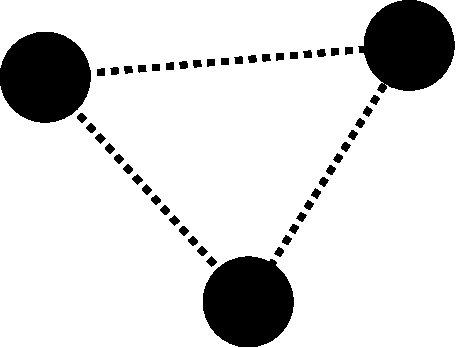
\includegraphics[height=3cm,width=4.5cm]{diagram-20210911(13)-crop}
	\end{figure}
	\begin{tasks}(4)
		\task[\textbf{A.}] $\frac{3}{2} k_{B}$
		\task[\textbf{B.}] $3 k_{B}$
		\task[\textbf{C.}] $\frac{9}{2} k_{B}$
		\task[\textbf{D.}] $6 k_{B}$
	\end{tasks}
	\begin{answer}
		If given molecules are at lower temperature i.e. atoms are attached to rigid rod then degree of freedom is 6 , so internal energy is $\frac{6 k_{B} T}{2}$, but at high temperature, vibration mode will active, so there are three extra vibration mode will active, so total energy
		\begin{align*}
		U&=3 k_{B} T+3 k_{B} T=6 k_{B} T\\
		C_{V}&=\left(\frac{\partial U}{\partial T}\right)_{V}=6 k_{B}
		\end{align*}
		So the correct answer is \textbf{Option (D)}
	\end{answer}	
	\item Consider $N$ non- interacting, distinguishable particles in a two-level system at temperature $T$. The energies of the levels are 0 and $\varepsilon$, where $\varepsilon>0$. In the high temperature limit $\left(k_{B} T>\varepsilon\right)$, what is the population of particles in the level with energy $\varepsilon ?$
	{\exyear{GATE 2017}}
	\begin{tasks}(4)
		\task[\textbf{A.}] $\frac{N}{2}$
		\task[\textbf{B.}] $N$
		\task[\textbf{C.}] $\frac{N}{4}$
		\task[\textbf{D.}] $\frac{3 N}{4}$
	\end{tasks}
	\begin{answer}
		\begin{align*}
		P(\varepsilon)&=\frac{\exp -\frac{\varepsilon}{k T}}{1+\exp -\frac{\varepsilon}{k T}},\text{ population of particle in the level with energy $\varepsilon$ is}\\
		N P(\varepsilon)&=N \frac{\exp -\frac{\varepsilon}{k T}}{1+\exp -\frac{\varepsilon}{k T}},\text{ for }\left(k_{B} T>\varepsilon\right), N P(\varepsilon)\\&=N \frac{\exp -\frac{\varepsilon}{k T}}{1+\exp -\frac{\varepsilon}{k T}}=N \frac{1}{1+1}=\frac{N}{2}
		\end{align*}
		So the correct answer is \textbf{Option (A)}
	\end{answer}	
	\item  A microcanonical ensemble consists of 12 atoms with each taking either energy 0 state, or energy $\in$ state. Both states are non-degenerate. If the total energy of this ensemble is $4 \in$, its entropy will be----------- $k_{B}$ (up to one decimal place), where $k_{B}$ is the Boltzmann constant.
	{\exyear{GATE 2018}}
	\begin{answer}
		\begin{align*}
		\intertext{The number of ways having total energy $4 \in$, out of 12 atom is}
		&={ }^{12} C_{4}=\frac{12}{\lfloor 48}=\frac{12 \times 11 \times 10 \times 9}{4 \times 3 \times 2}=495\\
		\text{Hence, entropy, }S&=k_{B} \ln w=k_{B} \ln (495)=k_{B}(6.204)=6.204 k_{B}
		\end{align*}
	\end{answer}	
	\item  The partition function of an ensemble at a temperature $T$ is
	$$
	Z=\left(2 \cosh \frac{\varepsilon}{k_{B} T}\right)^{N}
	$$
	where $k_{B}$ is the Boltzmann constant. The heat capacity of this ensemble at $T=\frac{\varepsilon}{k_{B}}$ is $X N k_{B}$, where the value of $X$ is (up to two decimal places).
	{\exyear{GATE 2018}}
	\begin{answer}
		\begin{align*}
		\text{	The partition function, }z&=\left[2 \cosh \left(\frac{\varepsilon}{k_{B} T}\right)\right]^{N}\\
		\text{The average energy, }\langle E\rangle&=k_{B} T^{2} \frac{\partial(\ln z)}{\partial T}\\
		&=\frac{N k_{B} T^{2}\left[2 \sinh \left(\frac{\varepsilon}{k_{B} T}\right)\right]\left(\frac{-\varepsilon}{k_{B} T^{2}}\right)}{2 \cosh \left(\frac{\varepsilon}{k_{B} T}\right)}\\&=-N \varepsilon \tanh \left(\frac{\varepsilon}{k_{B} T}\right)\\
		C&=\frac{d\langle E\rangle}{d T}=-N \varepsilon \sec h^{2}\left(\frac{\varepsilon}{k_{B} T}\right) \cdot\left(\frac{-\varepsilon}{k_{B} T^{2}}\right)\\
		\text{At }T&=\frac{\varepsilon}{k}, C=\frac{N \varepsilon^{2}}{k \cdot\left(\varepsilon^{2} / k^{2}\right)} \sec h^{2}(1)\\&=N k \sec h^{2}(1)=0.42 N k_{B}
		\end{align*}
	\end{answer}	
	\item A collection of $N$ two-level systems with energies 0 and $E>0$ is in thermal
	equilibrium at temperature $T$. For $T \rightarrow \infty$, the specific heat approaches to,
	{\exyear{JEST 2012}}
	\begin{tasks}(4)
		\task[\textbf{A.}] 0
		\task[\textbf{B.}] $N k_{B}$
		\task[\textbf{C.}] $\frac{3 N k_{B}}{2}$
		\task[\textbf{D.}] $\infty$
	\end{tasks}
	\begin{answer}
		\begin{align*}
		Z&=\sum e^{-\beta E_{i}}=e^{-\beta \times 0}+e^{-\beta E_{i}} \Rightarrow Z\\&=1+e^{-\beta E} \Rightarrow \ln z\\&=\ln \left(1+e^{-\beta E}\right)\\
		U&=\langle E\rangle=-\frac{\partial}{\partial \beta} \ln z\\&=-\frac{\partial}{\partial \beta} \ln \left(1+e^{-\beta E}\right)\\&=-\frac{1}{1+e^{-\beta E}} \times e^{-\beta E}(-E)\\&=\frac{E e^{-\beta E}}{1+e^{-\beta E}}\\
		\text{Now},\left(\frac{\partial U}{\partial T}\right)_{V}&=C_{V}\\
		&=\frac{\partial}{\partial T}\left(\frac{E e^{-\frac{E}{k T}}}{1+e^{-\frac{E}{k T}}}\right)\\
		\Rightarrow C_{V}&=\frac{\left(\frac{E^{2}}{k T^{2}} e^{\frac{-E}{k T}}+\frac{E^{2}}{k T^{2}} e^{\frac{-2 E}{k T}}-\frac{E^{2}}{k T^{2}} e^{\frac{-2 E}{k T}}\right)}{\left(1+e^{\frac{-E}{k T}}\right)^{2}} \Rightarrow C_{V}\\
		&=\left.\frac{\frac{E^{2}}{k T^{2}} e^{\frac{-E}{k T}}}{\left(1+e^{\frac{-E}{k T}}\right)^{2}} \Rightarrow C_{V}\right|_{T \rightarrow \infty}=0
		\end{align*}
		So the correct answer is \textbf{Option (A)}
	\end{answer}	
	\item  A monoatomic gas consists of atoms with two internal energy levels, ground state $E_{0}=0$ and an excited state $E_{1}=E$. The specific heat of the gas is given by
	{\exyear{JEST 2014}}
	\begin{tasks}(2)
		\task[\textbf{A.}] $\frac{3}{2} k$
		\task[\textbf{B.}] $\frac{E^{2} e^{E / k T}}{k T^{2}\left(1+e^{E / k T}\right)^{2}}$
		\task[\textbf{C.}] $\frac{3}{2} k+\frac{E^{2} e^{E / k T}}{k T^{2}\left(1+e^{E / k T}\right)^{2}}$
		\task[\textbf{D.}] $\frac{3}{2} k-\frac{E^{2} e^{E / k T}}{k T^{2}\left(1+e^{E / k T}\right)^{2}}$
	\end{tasks}
	\begin{answer}
		\begin{align*}
		E_{0}&=0, \quad E_{1}=E\\
		\text{Then partition function is}\\
		z&=\sum e^{-\beta E_{i}} \Rightarrow z\\&=e^{-\beta \times 0}+e^{-\beta E} \Rightarrow \ln z\\&=\ln \left(1+e^{-\beta E_{1}}\right)\\
		U&=\langle E\rangle=\frac{-\partial}{\partial \beta} \ln z\\&=-\frac{\partial}{\partial \beta} \ln \left(1+e^{-\beta E}\right)\\&=-\frac{1}{\left(1+e^{-\beta E}\right)}(-E) e^{-\beta E}\\&=\frac{E e^{-\beta E}}{1+e^{-\beta E}} \quad\left[\because \beta=k_{B} T\right]\\
		\left(\frac{\partial U}{\partial T}\right)_{v}=C_{V}&=\frac{\left(1+e^{-\frac{E}{k_{B} T}}\right) E . e^{-\frac{E}{k_{B} T}} \cdot\left(\frac{E}{k_{B} T^{2}}\right)-E e^{-\frac{E}{k_{B} T}} \cdot e^{-\frac{E}{k_{B} T}}\left(\frac{E}{k_{B} T^{2}}\right)}{\left(1+e^{-\frac{E}{k_{B} T}}\right)^{2}}\\
		C_{V}&=\frac{\frac{E^{2}}{k_{B} T^{2}} e^{-\frac{E}{k_{\mathrm{B}} T}}+\frac{E^{2}}{k_{B} T^{2}} e^{-\frac{2 E}{k_{\mathrm{B}} T}}-\frac{E^{2}}{k_{B} T^{2}} e^{-\frac{2 E}{k_{\mathrm{B}} T}}}{\left(1+e^{-\frac{E}{k_{\mathrm{B}} T}}\right)^{2}}\\&=\frac{E^{2} e^{-\frac{E}{k_{\mathrm{B}} T}}}{k_{B} T^{2}\left(1+e^{-\frac{E}{k_{\mathrm{B}} T}}\right)^{2}}\\&=\frac{E^{2} e^{\frac{E}{k_{\mathrm{B}} T}}}{k_{B} T^{2}\left(1+e^{\frac{E}{k_{\mathrm{B}} T}}\right)^{2}}\\
		\text{If gas will classically allowed, then }C_{V}&=\frac{3}{2} k_{B}\\
		\text{	and quantum mechanically, }C_{V}&=\frac{E^{2} e^{\frac{E}{k_{B} T}}}{k_{B} T^{2}\left(1+e^{\frac{E}{k_{B} T}}\right)^{2}}\\
		\therefore \quad C_{V}&=\frac{3}{2} k_{B}+\frac{E^{2} e^{E / k T}}{k T^{2}\left(1+e^{E / k T}\right)^{2}}
		\end{align*}
		So the correct answer is \textbf{Option (C)}
	\end{answer}	
	\item Consider a system of $2 N$ non-interacting spin $1 / 2$ particles each fixed in position and carrying a magnetic moment $\mu$. The system is immersed in a uniform magnetic field $B$. The number of spin up particles for which the entropy of the system will be maximum is
	{\exyear{JEST 2014}}
	\begin{tasks}(4)
		\task[\textbf{A.}]  0
		\task[\textbf{B.}] $N$
		\task[\textbf{C.}] $2 N$
		\task[\textbf{D.}] $N / 2$
	\end{tasks}
	\begin{answer}
		\begin{align*}
		\intertext{Let us consider $n$ number of spin out of $2 N$ particle have spin up remaining $2 N-n$ is down.}
		\text{Number of ways, }\omega&=\left\{\begin{array}{ll}2^{N} C_{n} & \text { for spin } \frac{1}{2}(\text { up }) \\ 2^{N} C_{2 N-n} & \text { for spin } \frac{1}{2}(\text { down })\end{array}\right.\\
		\text{Entropy, }S&=k \ln \omega \Rightarrow S\\&=k \ln { }^{2 N} C_{2 N-n}+k \ln { }^{2 N} C_{n}\\
		S&=k\left\{\left[\ln \frac{2 N !}{(n !)(2 N-n) !}\right]+\left[\ln \frac{2 N !}{(n !)(2 N-n) !}\right]\right\}\\
		S&=2 k[(\ln 2 N !-\ln n !-\ln (2 N-n) !)]\\
		S&=2 k[2 N \ln 2 N-2 N-n \ln n+n-\{(2 N-n) \ln (2 N-n)-(2 N-n)\}]\\
		[\because \ln N !&=N \ln N-N !]\\
		S&=2 k[2 N \ln 2 N-2 N-n \ln n+n-2 N \ln (2 N-n)+n \ln (2 N-n)+(2 N-n)]\\
		S&=2 k[2 N \ln 2 N-n \ln n-2 N \ln (2 N-n)+n \ln (2 N-n)]
		\intertext{Now for maximum entropy at equilibrium for spin $\frac{1}{2}$ up particle,}
		\frac{d S}{d n}&=0\\
		\frac{d S}{d n}&=2 k\left[-\frac{n}{n} \cdot 1-\ln n-\frac{2 N}{2 N-n}(-1)+\frac{n}{2 N-n}(-1)+\ln (2 N-n)\right]\\
		&=2 k\left[-1-\ln n+\frac{2 N}{2 N-n}-\frac{n}{2 N-n}+\ln (2 N-n)\right]\\
		&=2 k\left[-1+\frac{2 N-n}{2 N-n}+\ln (2 N-n)-\ln n\right]\\& \Rightarrow 2 k\left[-1+1+\ln \frac{(2 N-n)}{n}\right]=0\\
		\because \quad 2 k &\neq 0\\
		\therefore \ln \left(\frac{2 N-n}{n}\right)&=0 \Rightarrow \frac{2 N-n}{n}\\&=1 \Rightarrow 2 N=2 n \\
		\Rightarrow n&=N
		\end{align*}
		So the correct answer is \textbf{Option (B)}
	\end{answer}	
	\item For a system in thermal equilibrium with a heat bath at temperature $T$, which one of the following equalities is correct? $\left(\beta=\frac{1}{k_{B} T}\right)$
	{\exyear{JEST 2015}}
	\begin{tasks}(2)
		\task[\textbf{A.}] $\frac{\partial}{\partial \beta}\langle E\rangle=\langle E\rangle^{2}-\left\langle E^{2}\right\rangle$
		\task[\textbf{B.}] $\frac{\partial}{\partial \beta}\langle E\rangle=\left\langle E^{2}\right\rangle-\langle E\rangle^{2}$
		\task[\textbf{C.}] $\frac{\partial}{\partial \beta}\langle E\rangle=\left\langle E^{2}\right\rangle+\langle E\rangle^{2}$
		\task[\textbf{D.}] $\frac{\partial}{\partial \beta}\langle E\rangle=-\left(\left\langle E^{2}\right\rangle+\langle E\rangle^{2}\right)$
	\end{tasks}
	\begin{answer}
		\begin{align*}
		\because\langle E\rangle&=\frac{\sum_{i} E_{i} e^{-\beta E_{i}}}{\sum_{i} e^{-\beta E_{i}}}\\
		\frac{\partial\langle E\rangle}{\partial \beta}&=-\frac{\sum_{i} E_{i}^{2} e^{-\beta E_{i}}}{\sum_{i} e^{-\beta E_{i}}}+\frac{\sum_{i} E_{i}^{2} e^{-\beta E_{i}} \cdot e^{-\beta E_{i}}}{\left(\sum_{i} e^{-\beta E_{i}}\right)^{2}}\\&=-\frac{\sum_{i} E_{i}^{2} e^{-\beta E_{i}}}{\sum_{i} e^{-\beta E_{i}}}+\frac{\sum_{i} E_{i}^{2} e^{-2 \beta E_{i}}}{\left(\sum_{i} e^{-\beta E_{i}}\right)^{2}}\\
		\Rightarrow \frac{\partial\langle E\rangle}{\partial \beta}&=\langle E\rangle^{2}-\left\langle E^{2}\right\rangle
		\end{align*}
		So the correct answer is \textbf{Option (A)}
	\end{answer}	
	\item A particle in thermal equilibrium has only 3 possible states with energies $-\in, 0, \in .$ If the system is maintained at a temperature, $T>>\frac{\epsilon}{k_{B}}$, then the average energy of the particle can be approximated to,
	{\exyear{JEST 2015}}
	\begin{tasks}(4)
		\task[\textbf{A.}] $\frac{2 \in^{2}}{3 k_{B} T}$
		\task[\textbf{B.}] $\frac{-2 \in^{2}}{3 k_{B} T}$
		\task[\textbf{C.}] $\frac{-\epsilon^{2}}{k_{B} T}$
		\task[\textbf{D.}]  0
	\end{tasks}
	\begin{answer}
		\begin{align*}
		\langle E\rangle&=\frac{-\in e^{+\frac{\epsilon}{k T}}+0+\in e^{-\frac{\epsilon}{k T}}}{e^{\frac{\epsilon}{k T}}+1+e^{-\frac{\epsilon}{k T}}}\\&=\epsilon\left(\frac{e^{-\frac{\epsilon}{k T}}-e^{\frac{\epsilon}{k T}}}{1+e^{-\frac{\epsilon}{k T}}+e^{\frac{\epsilon}{k T}}}\right)\\
		\Rightarrow\langle E\rangle&=\frac{\left[\left(1-\frac{\epsilon}{k T}\right)-\left(1+\frac{\epsilon}{k T}\right)\right]}{1+\left(1-\frac{\epsilon}{k T}\right)+\left(1+\frac{\epsilon}{k T}\right)}\\&=\frac{-2 \epsilon^{2}}{3 k T}
		\end{align*}
		So the correct answer is \textbf{Option (B)}
	\end{answer}	
	\item A collection of $N$ interacting magnetic moments, each of magnitude $\mu$, is subjected to a magnetic field $\mathrm{H}$ along the $\mathrm{z}$ direction. Each magnetic moment has a doubly degenerate level of energy zero and two non-degenerate levels of energies $-\mu H$ and $\mu H$ respectively.The collection is in thermal equilibrium at temperature $T$. The total energy $E(T, H)$ of the collection is
	{\exyear{JEST 2018}}
	\begin{tasks}(2)
		\task[\textbf{A.}] $-\frac{\mu H N \sinh \left(\frac{\mu H}{k_{B} T}\right)}{1+\cosh \left(\frac{\mu H}{k_{b} T}\right)}$
		\task[\textbf{B.}] $-\frac{\mu H N}{2\left(1+\cosh \left(\frac{\mu H}{k_{b} T}\right)\right)}$
		\task[\textbf{C.}] $-\frac{\mu H N \cosh \left(\frac{\mu H}{k_{B} T}\right)}{1+\cosh \left(\frac{\mu H}{k_{b} T}\right)}$
		\task[\textbf{D.}] $-\mu H N \frac{\sinh \left(\frac{\mu H}{k_{B} T}\right)}{\cosh \left(\frac{\mu H}{k_{b} T}\right)}$
	\end{tasks}
	\begin{answer}
		\begin{align*}
		Z_{1}&=\left(2 \times \exp \left(-\frac{0}{k_{B} T}\right)+\exp \left(-\frac{-\mu H}{k_{B} T}\right)+\exp \left(-\frac{\mu H}{k_{B} T}\right)\right) \\\Rightarrow Z_{1}&=\left(2+2 \cosh \frac{\mu H}{k_{B} T}\right)\\
		Z_{N}&=\left(2+2 \cosh \frac{\mu H}{k_{B} T}\right)^{N}\\U&=k_{B} T^{2}\left(\frac{\partial \ln Z_{N}}{\partial T}\right)_{N, V}\\&=-\frac{N \mu H \sinh \left(\frac{\mu H}{k_{B} T}\right)}{1+\cos \frac{\mu H}{k_{B} T}}
		\end{align*}
		So the correct answer is \textbf{Option (A)}
	\end{answer}
	\item 	Consider a system of $N$ distinguishable particles with two energy levels for each particle, a ground state with energy zero and an excited state with energy $\varepsilon>0$. What is the average energy per particle as the system temperature $T \rightarrow \infty$ ?
	{\exyear{JEST 2019}}
	\begin{tasks}(4)
		\task[\textbf{A.}] 0
		\task[\textbf{B.}]  $\frac{\varepsilon}{2}$
		\task[\textbf{C.}] $\varepsilon$
		\task[\textbf{D.}] $\infty$
	\end{tasks}
	\begin{answer}
		\begin{align*}
		\langle E\rangle&=\sum_{i} P_{i} E_{i} \Rightarrow P_{i}=\frac{e^{\beta E_{i}}}{z}\\
		\langle E\rangle&=0 \times \frac{01}{1+e^{-\beta \varepsilon}}+\varepsilon \times \frac{1}{1+e^{-\beta \varepsilon}}\\
		&=\frac{\varepsilon}{1+e^{-\varepsilon / k_{B} T}}=\frac{\varepsilon}{2}\text{`}T \rightarrow \infty
		\end{align*}
		So the correct answer is \textbf{Option (B)}
	\end{answer}
	\item Consider a diatomic molecule with an infinite number of equally spaced non-degenerate energy levels. The spacing between any two adjacent levels is $\varepsilon$ and the ground state energy is zero. What is the single particle partition function $Z$ ?
	{\exyear{JEST 2019}}
	\begin{tasks}(2)
		\task[\textbf{A.}] $Z=\frac{1}{1-\frac{\varepsilon}{k_{B} T}}$
		\task[\textbf{B.}] $Z=\frac{1}{1-e^{\frac{\varepsilon}{k_{\mathrm{B}} T}}}$
		\task[\textbf{C.}] $Z=\frac{1}{1-e^{\frac{2 \varepsilon}{k_{B} T}}}$
		\task[\textbf{D.}] $Z=\frac{1-\frac{\varepsilon}{k_{B} T}}{1+\frac{\varepsilon}{k_{B} T}}$
	\end{tasks}
	\begin{answer}
		\begin{align*}
		Z&=\sum_{i} g_{i} e^{-\beta \varepsilon_{i}}\\
		g_{i}&=1\\
		Z&=1+e^{-\beta \varepsilon}+e^{-2 \beta \varepsilon}+\ldots \ldots\\
		Z&=\frac{1}{1-e^{-\beta \varepsilon}}
		\end{align*}
		No option is matched
	\end{answer}	
\end{enumerate}